\section{Discussion}\label{sec:discussion}

According to Table~\ref{tab:prcurves}, the best results were obtained by Rprop-NoComp, Clus-HMC and Clus-HSC. We can see that using the true classes to augment the feature vectors did not improve the classification results when compared to the HMC-LMLP version that does not use the augmentation process. We believe there are two reasons that may have harmed Bp(Rprop)-Comp's performance: (i) adapting the DAG hierarchy, and (ii) using different values to augment the feature vectors during the training and test phases.

Regarding the adaptation made in the DAG hierarchies, Bp-Comp and Rprop-Comp could have achieved better performance if all relationships between classes had been available during training. Recall we had to adapt the DAG hierarchy to define the depth of a class as being the number of edges in the longest path between class and root node. For that reason, many hierarchical relationships between classes were not considered during the training phase. Figure~\ref{fig:hrelationships} illustrates a scenario that explains this rationale.

\begin{figure}[htbp]
       \centering
       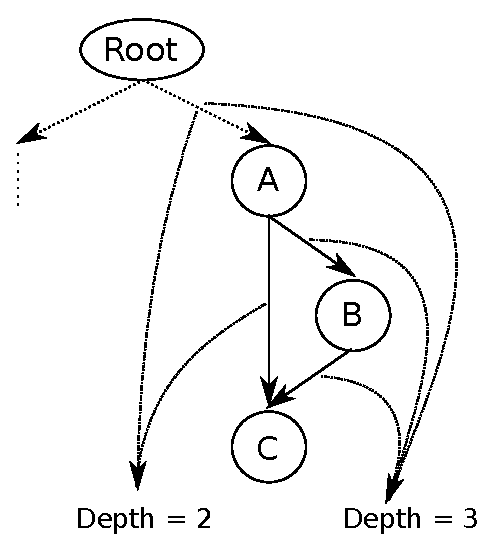
\includegraphics[scale=0.5]{hrelationships}
       \caption{Illustrative example of different depths for the same class.}
       \label{fig:hrelationships}
\end{figure}

Following the scenario presented in Figure~\ref{fig:hrelationships}, consider that a training instance is assigned to paths A.C and A.B.C, and that class C is a direct subclass of both classes A and B. In this scenario, there are two possible depths for class C: 2 (A.C) and 3 (A.B.C). In the adaptation process we have proposed, class C is defined as belonging to the third level. In this case, when training an MLP for the third level, we consider class C as subclass of class B alone. Thus, when training a neural network to predict class C (third level), we are not using the information related to all its superclasses (classes A and B) as inputs. Only class B is considered.

The different values that are used when augmenting the feature vectors may also have harmed the performance of Bp-Comp and Rprop-Comp. Recall that when training an MLP for level $l$, we make use of the true labels of the training instances (values 0 or 1) at level $l-1$ to augment their feature vectors. However, the true labels are not available during test. Thus, the predictions made by the neural network at level $l-1$ (values [0,1]) were used instead. Therefore, each MLP was trained using 0 or 1 values for augmenting the feature vectors during training, but were tested with real values in the interval [0,1].

Comparing the Bp and Rprop algorithms, note that the Rprop versions of HMC-LMLP provided better predictive performance than the Bp versions. These results suggest that Rprop copped better with the greater number of attributes, which increased considerably due to the augmentation process. 

\begin{figure}[!htpb]
 \centering 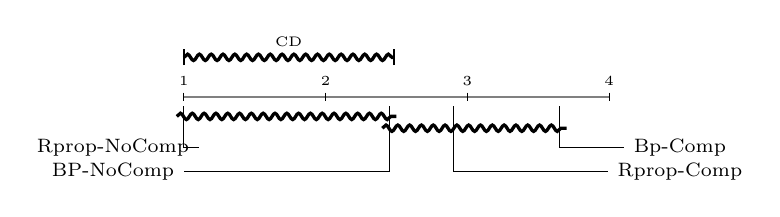
\begin{tikzpicture}[xscale=1.8]
\node (Label) at  (01.7400,0.7) {\tiny{CD}}; % the label
\draw[decorate,decoration={snake,amplitude=.4mm,segment length=1.5mm,post length=0mm}, very thick, color = black](01.0000, 0.5) -- (02.4800, 0.5);
\foreach \x in {01.0000,02.4800} \draw[thick,color = black] (\x, 0.4) -- (\x, 0.6);

\draw[gray, thick](01.0000, 0) -- (04.0000, 0);
\foreach \x in {01.0000,02.0000,03.0000,04.0000}\draw (\x cm,1.5pt) -- (\x cm, -1.5pt);
\node (Label) at (01.0000,0.2) {\tiny{1}};
\node (Label) at (02.0000,0.2) {\tiny{2}};
\node (Label) at (03.0000,0.2) {\tiny{3}};
\node (Label) at (04.0000,0.2) {\tiny{4}};
\draw[decorate,decoration={snake,amplitude=.4mm,segment length=1.5mm,post length=0mm}, very thick, color = black](00.9500,-00.2500) -- ( 02.5000,-00.2500);
\draw[decorate,decoration={snake,amplitude=.4mm,segment length=1.5mm,post length=0mm}, very thick, color = black](02.4000,-00.4000) -- ( 03.7000,-00.4000);
\node (Point) at (01.0000, 0){};  \node (Label) at (0.5,-00.6500){\scriptsize{Rprop-NoComp}}; \draw (Point) |- (Label);
\node (Point) at (02.4500, 0){};  \node (Label) at (0.5,-00.9500){\scriptsize{BP-NoComp}}; \draw (Point) |- (Label);
\node (Point) at (03.6500, 0){};  \node (Label) at (4.5,-00.6500){\scriptsize{Bp-Comp}}; \draw (Point) |- (Label);
\node (Point) at (02.9000, 0){};  \node (Label) at (4.5,-00.9500){\scriptsize{Rprop-Comp}}; \draw (Point) |- (Label);
\end{tikzpicture}
\caption{Critical diagram presenting results of the 4 HMC-LMLP's versions.}
\label{fig:cdNN}
\end{figure}

Figure~\ref{fig:cdNN} shows the results of the statistical tests regarding the 4 HMC-LMLP's versions. Note that Rprop-NoComp outperforms most versions of HMC-LMLP with statistical significance. The difference for BP-NoComp is within the limit of the critical difference. The tests confirm that Rprop was the best learning algorithm in both scenarios (with and without augmentation). 


Figure~\ref{fig:cdAll} presents the results of the statistical tests regarding the best version of HMC-LMLP (Rprop-NoComp) and the 4 baseline methods (Clus-HMC, Clus-HSC, Clus-SC, and \textit{hm}Ant-Miner). Clus-HMC provides the lowest average rank (2.0), whereas Rprop-NoComp provides the second lowest (2.15) followed by Clus-HSC (2.25). Note that the difference in average rank among these three methods is very small, and indeed it is deemed as insignificant by the statistical tests. The performance achieved by \textit{hm}Ant-Miner (average rank of 3.6) and Clus-SC (average rank of 5.0) is considerably lower than the best ranked methods. Even though \textit{hm}Ant-Miner is within the limit of the critical difference, Clus-SC is out of the significance margin, which means it is outperformed by the first three methods with statistical significance.

\begin{figure}[!htpb]
 \centering 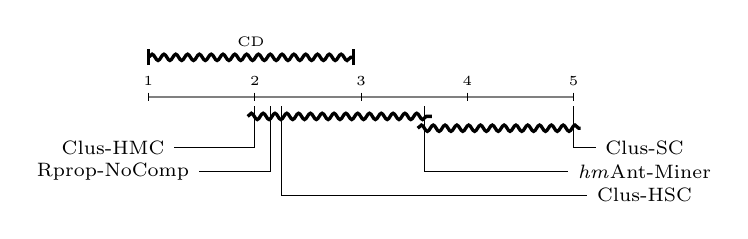
\begin{tikzpicture}[xscale=1.8]
\node (Label) at  (01.4734,0.7) {\tiny{CD}}; % the label
\draw[decorate,decoration={snake,amplitude=.4mm,segment length=1.5mm,post length=0mm}, very thick, color = black](00.7500, 0.5) -- (02.1967, 0.5);
\foreach \x in {00.7500,02.1967} \draw[thick,color = black] (\x, 0.4) -- (\x, 0.6);

\draw[gray, thick](00.7500, 0) -- (03.7500, 0);
\foreach \x in {00.7500,01.5000,02.2500,03.0000,03.7500}\draw (\x cm,1.5pt) -- (\x cm, -1.5pt);
\node (Label) at (00.7500,0.2) {\tiny{1}};
\node (Label) at (01.5000,0.2) {\tiny{2}};
\node (Label) at (02.2500,0.2) {\tiny{3}};
\node (Label) at (03.0000,0.2) {\tiny{4}};
\node (Label) at (03.7500,0.2) {\tiny{5}};
\draw[decorate,decoration={snake,amplitude=.4mm,segment length=1.5mm,post length=0mm}, very thick, color = black](01.4500,-00.2500) -- ( 02.7500,-00.2500);
\draw[decorate,decoration={snake,amplitude=.4mm,segment length=1.5mm,post length=0mm}, very thick, color = black](02.6500,-00.4000) -- ( 03.8000,-00.4000);
\node (Point) at (01.5000, 0){};  \node (Label) at (0.5,-00.6500){\scriptsize{Clus-HMC}}; \draw (Point) |- (Label);
\node (Point) at (01.6125, 0){};  \node (Label) at (0.5,-00.9500){\scriptsize{Rprop-NoComp}}; \draw (Point) |- (Label);
\node (Point) at (03.7500, 0){};  \node (Label) at (4.25,-00.6500){\scriptsize{Clus-SC}}; \draw (Point) |- (Label);
\node (Point) at (02.7000, 0){};  \node (Label) at (4.25,-00.9500){\scriptsize{\textit{hm}Ant-Miner}}; \draw (Point) |- (Label);
\node (Point) at (01.6875, 0){};  \node (Label) at (4.25,-01.2500){\scriptsize{Clus-HSC}}; \draw (Point) |- (Label);
\end{tikzpicture}
\caption{Critical diagram presenting results of the best HMC-LMLP network and the baseline algorithms.}
\label{fig:cdAll}
\end{figure}

Considering the results in specific classes (Table~\ref{tab:classesSeq}), HMC-LMLP provided the best results in the great majority of the classes. These results are quite unexpected, given that Clus-HMC achieved a better overall performance than Bp-Comp, Bp-NoComp and Rprop-Comp (Table~\ref{tab:prcurves}). Notwithstanding, we verified that from the 2849 classes that belong to the test dataset, Clus-HMC provided the best results for 2192, whereas the HMC-LMLP's versions achieved the best results in a much smaller number of classes. Hence the results of Clus-HMC in Table~\ref{tab:prcurves}.

The PR-curves obtained for datasets Eisen and Seq are depicted in Figure~\ref{fig:prcurves}. These datasets are the ones where Clus-HMC obtained its best results. We compared the PR-curves of the literature methods with the PR-curve obtained by Rprop-NoComp, since it was the best among the HMC-LMLP's versions. The PR-curves shown for HMC-LMLP and {\it hm}Ant-Miner are those from the executions in which they obtained the best results in the validation data. We can see that Clus-HMC, Clus-HSC and HMC-LMLP are quite even performance-wise.

\begin{figure*}[ht]
        \centering
        \begin{subfigure}[b]{0.3\textwidth}
                \centering
                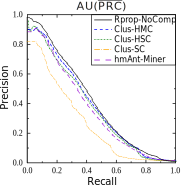
\includegraphics[scale=1.1]{eisen}
                \caption{Eisen dataset}
                \label{fig:eisenTree}
        \end{subfigure}
		\qquad\qquad\qquad
        \begin{subfigure}[b]{0.3\textwidth}
                \centering
                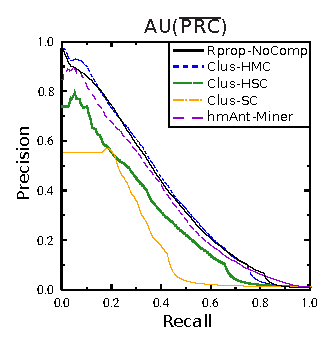
\includegraphics[scale=1.1]{seq}
                \caption{Seq dataset}
                \label{fig:seqTree}
        \end{subfigure}
        \caption{PR-curves of Rprop-NoComp, Clus-HMC, CLus-HSC, Clus-SC, and {\it hm}Ant-Miner.}
        \label{fig:prcurves}
\end{figure*}